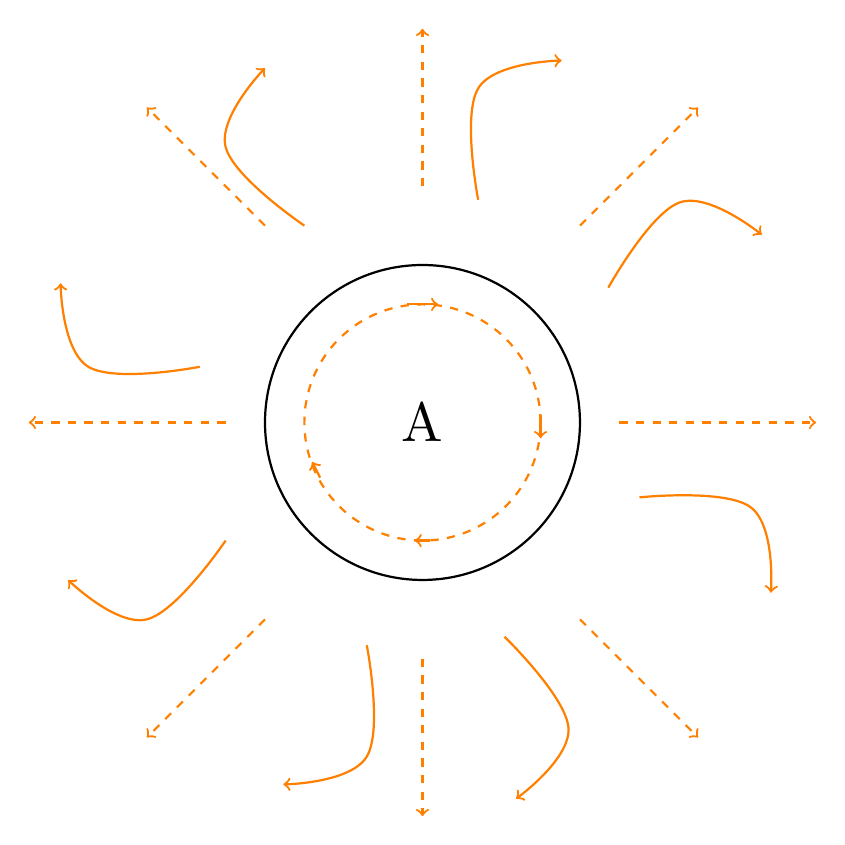
\begin{tikzpicture}

\draw  [thick](0,0) circle (2);
\draw [thick, ->, dashed, orange](-2,2.5) -- (-3.5,4);
\draw [thick, ->, dashed, orange] (-2,-2.5) -- (-3.5,-4);
\draw [thick, ->, dashed, orange] (2,2.5) -- (3.5,4);
\draw [thick, ->, dashed, orange] (2,-2.5) -- (3.5,-4);
\draw [thick, ->, dashed, orange] (2.5,0) -- (5,0);
\draw [thick, ->, dashed, orange] (-2.5,0) -- (-5,0);
\draw [thick, ->, dashed, orange] (0,3) -- (0,5);
\draw [thick, ->, dashed, orange] (0,-3) -- (0,-5);
\draw  [->, thick, orange]plot[smooth, tension=.7] coordinates{(-1.5,2.5) (-2.5,3.5) (-2,4.5)};
\draw  [->, thick, orange] plot[smooth, tension=.7, rotate=45] coordinates{(-1.5,2.5) (-2.5,3.5) (-2,4.5)};
\draw [->, thick, orange]  plot[smooth, tension=.7, rotate=90] coordinates{(-1.5,2.5) (-2.5,3.5) (-2,4.5)};
\draw  [->, thick, orange] plot[smooth, tension=.7, rotate=135] coordinates {(-1.5,2.5) (-2.5,3.5) (-2,4.5)};
\draw   [->, thick, orange]plot[smooth, tension=.7, rotate=170] coordinates {(-1.5,2.5) (-2.5,3.5) (-2,4.5)};
\draw [->, thick, orange]  plot[smooth, tension=.7, rotate=220] coordinates {(-1.5,2.5) (-2.5,3.5) (-2,4.5)};
\draw [->, thick, orange]  plot[smooth, tension=.7, rotate=275] coordinates{(-1.5,2.5) (-2.5,3.5) (-2,4.5)};
\draw  [->, thick, orange] plot[smooth, tension=.7, rotate=-45] coordinates {(-1.5,2.5) (-2.5,3.5) (-2,4.5)};
\node [scale=2] (v1) at (0,0) {A};
\draw  [dashed, orange, thick](v1) circle (1.5);
\draw [<-, orange, thick](-1.4,-0.5) -- (-1.3,-0.7);
\draw [<-, orange, thick] (-0.1,-1.5) -- (0.1,-1.5);
\draw  [<-, orange, thick](1.5,-0.2) -- (1.5,0.1);
\draw [<-, orange, thick] (0.2,1.5) -- (-0.2,1.5);
\end{tikzpicture}